\documentclass[11pt,a4paper]{article}
\usepackage[utf8]{inputenc}
\usepackage[spanish]{babel}
\usepackage{amsmath,amssymb,amsthm,mathtools,enumitem,microtype}
\renewcommand{\refname}{Referencias}
\usepackage[a4paper,margin=2.5cm]{geometry}
\usepackage[dvipsnames]{xcolor}
\usepackage[most]{tcolorbox}
\bibliographystyle{abbrvnat}
\usepackage[]{natbib}
\usepackage{tikz}
\usepackage[colorlinks=true,linkcolor=NavyBlue,urlcolor=NavyBlue,citecolor=NavyBlue]{hyperref}

\setlength{\parskip}{4pt}\setlength{\parindent}{0pt}
\setlist{itemsep=1pt,topsep=3pt}

% ---- ecuaciones destacadas
\newtcolorbox{eqbox}{colback=blue!4,colframe=blue!45!black,boxrule=0.5pt,arc=2pt,
  left=6pt,right=6pt,top=2pt,bottom=2pt,before skip=6pt,after skip=6pt}
\newtcolorbox{nota}{colback=yellow!12,colframe=orange!60!black,boxrule=0.5pt,arc=2pt,
  left=6pt,right=6pt,top=4pt,bottom=4pt,before skip=8pt,after skip=8pt}

% ---- teoremas
\theoremstyle{plain}
\newtheorem{lema}{Lema}[section]
\newtheorem{proposicion}[lema]{Proposición}
\newtheorem{corolario}[lema]{Corolario}
\theoremstyle{definition}
\newtheorem{definicion}[lema]{Definición}
\theoremstyle{remark}
\newtheorem{observacion}[lema]{Observación}

% ---- notación
\newcommand{\R}{\mathbb{R}}
\newcommand{\Z}{\mathbb{Z}}
\newcommand{\one}{\mathbf{1}}
\newcommand{\Hs}{\mathcal{H}}          % Hessiano
\newcommand{\Tn}{\mathcal{T}}          % aristas en tensión
\newcommand{\Rs}{\mathcal{R}}          % aristas relajadas
\newcommand{\Nn}{\mathcal{N}}          % matriz C^{1/2} M C^{1/2}
\newcommand{\Kn}{\mathcal{K}}          % vecinos comunes de un triple
\newcommand{\etq}[1]{\textsf{\small[#1]}}
\newcommand{\propio}{\etq{propio$^*$}}
\newcommand{\lit}{\etq{literatura}}
\newcommand{\aqui}{\etq{demostrado aquí}}

\title{\textbf{Kuramoto desde la topología}}
\author{Manuel Ferro, Lucas Grasso Ramos,Tomás Brucellaria, Tadeo Solari}
\date{}

\begin{document}

\maketitle

\section{Modelo de Kuramoto}
La energía elástica total y el modelo de Kuramoto \citep{10.1007/BFb0013365} son:
\begin{eqbox}\[
E(\theta)=\sum_{\{a,b\}\in E}\bigl(1-\cos(\theta_a-\theta_b)\bigr),\qquad
\dot\theta_u=-\frac{\partial E}{\partial\theta_u}=\sum_{v\sim u}\sin(\theta_v-\theta_u),
\]\end{eqbox}
Llamamos a un equilibrio  $desincronizado$ si es un mínimo local que no coincide con el global. El sistema será $desincronizado$ cuando haya mínimos desincronizados estables. En caso contrario, ambos son $sincronizados$. 

Del mismo modo, con $\delta=\min_v\deg v$, se define la conectividad como: 
\begin{eqbox}\[
\mu(G):=\frac{\delta+1}{n}.
\]\end{eqbox}

Y la conectividad critica como:
\begin{eqbox}\[
\mu_c:=\inf\bigl\{\mu\in[0,1]:\ \text{todo }G\in\mathcal G\text{ con }\mu(G)\ge\mu\text{ es sincronizante}\bigr\}.
\]\end{eqbox}

\section{¿Por qué topología?}
Partamos de un ejemplo simple. No es complicado demostrar que todo grafo camino sincroniza, y sin embargo, al agregar una sola arista y hacerlo un grafo ciclo, ya no lo hace. Esto sugiere que la presencia de ciclos es la cualidad topológica determinante en la sincronización global. Con el fin de cuantificar este fenómeno, recurrimos a las nociones de \textit{winding number} \(q\) y los \(q\)\textit{-twisted states}.

\paragraph{Diferencia de fase envuelta.} Una arista $\{a,b\}$ es \emph{antípoda} si
$\theta_b-\theta_a\equiv\pi \pmod{2\pi}$. Si no lo es, podemos definir
$wrap(\theta)\in[-\pi,\pi)$ con \(wrap(\theta) = (\theta + \pi) \text{ mod } 2\pi - \pi\).

\paragraph{\textit{Winding} de un ciclo.} Para un ciclo $\mathcal{C}=(v_0\to v_1\to\dots\to v_k=v_0)$ en $G$ sin aristas antípodas, definimos:
\begin{eqbox}\[
q(\mathcal{C})=\frac1{2\pi}\sum_{i=0}^{k-1}wrap(\theta{v_{i+1}} - \theta{v_i})\in \mathbb{Z} .
\]\end{eqbox}
Dada una base de ciclos \(\mathcal{B} =\{ \mathcal{C}_1, \mathcal{C}_2, \cdots, \mathcal{C}_n\}\),
\begin{equation}
    \vec{q_\mathcal{B}} = (q(\mathcal{C}_1), q(\mathcal{C}_2), \cdots, q(\mathcal{C}_n))
\end{equation}

La sincronización del grafo es independiente a la base \(\mathcal{B}\) elegida. Con este enfoque planteamos el primer lema:

\begin{lema}[]
Sea $\theta$ un equilibrio de un grafo conexo, sin aristas antípodas. Entonces
\[
\vec{q}\equiv0\iff\theta\text{ es sincronizado}.
\]
\end{lema}



Intuitivamente, en un equilibrio sincronizado la diferencia de fases $\Delta\theta_e$ es nula en toda arista, lo que impide que el \(\vec{q}\) alcance valores enteros no nulos. Como línea de investigación futura, resulta de interés analizar la sensibilidad de $\Vert{}\vec{q}\Vert{}$ frente al cambio de la base de ciclos $Y$ y bajo la elección de distintas normas. La demonstracion de este y todos los lemas se encuentra en el repositorio adjunto, ver Sección~\ref{da}.



\section{Estabilidad desde las fases}
Sea $B$ la matriz de incidencia del grafo, su Hessiano resulta:


\begin{equation}
    \Hs(\theta^*) = B D B^T \quad \text{donde} \quad D = diag(\gamma_e) \qquad \gamma_e = cos(\Delta{\theta_e)}
\end{equation}

\cite{bronski2015graphhomologystabilitycoupled}.

Este hecho nos empujó a pensar la estabilidad desde los cosenos: si alguno fuera 0, es decir, si alguna arista estuviese uniendo vértices un cuarto de vuelta desfasados, el criterio fallaría y la estabilidad pasaría a depender de factores no lineales. Esto es debido a que el problema deja de ser definido positivo.

En la literatura se han referido a estas aristas como \emph{cortas} y \emph{largas}; nosotros preferimos usar otra nomenclatura:
\paragraph{Aristas relajadas y en tensión.} Dado un equilibrio, sean
\begin{eqbox}\[
\Rs=\{e:\gamma_e>0\},\qquad \Tn=\{e:\gamma_e\le 0\}.
\]\end{eqbox}
Entonces las aristas en $\Rs$ son aquellas que comunican vértices en clústeres de fase, estando \emph{relajadas}. Las de $\Tn$ son las interclústeres, siempre en \emph{tensión} si es que estos se mantienen separados en el equilibrio.

Notar que $\Hs=L_\Rs-L_\Tn$, donde $L_\Rs$ y $L_\Tn$ son los Laplacianos de $\Rs$ y $\Tn$ con pesos $|\gamma_e|$. Para vincular el conjunto $\Tn$ con el vector $\vec{q}$, definimos:

\paragraph{Cubrimientos ternarios.} 

Se seleccionan tres vértices en el círculo de fases tales que el triángulo determinado por sus posiciones contenga el centro de la circunferencia; denominamos a este conjunto cubrimiento ternario $S$. 

\begin{figure}[htbp]
    \centering

    \begin{center}
    \begin{tikzpicture}[scale=0.7]
    % 1. Dibujar el círculo
    \draw[thick, gray!70] (0,0) circle (2);

    % 2. Centro
    \filldraw[black] (0,0) circle (1.5pt);

    % 3. Coordenadas de los puntos
    \coordinate (P1) at (0:2);
    \coordinate (P2) at (100:2);
    \coordinate (P3) at (220:2);

    % 4. Triángulo
    \draw[thick, PosterHeading] (P1) -- (P2) -- (P3) -- cycle;

    % 5. Puntos coloreados y etiquetas
    \filldraw[blue!70!black]   (P1) circle (2.5pt) node[right=3pt] {$\phi_1$};
    \filldraw[orange!85!black] (P2) circle (2.5pt) node[above=3pt] {$\phi_2$};
    \filldraw[green!60!black]  (P3) circle (2.5pt) node[below left=3pt] {$\phi_3$};
\end{tikzpicture}
\end{center}

    \caption{Cubrimiento ternario $S=\{\phi_1, \phi_2, \phi_3\}$.}
    \label{fig:c4}
\end{figure}


Notar que, dado que el triángulo contiene al origen, la dispersión angular garantiza que cada vértice en $\mathcal{N}$ incida en al menos una arista perteneciente a $\mathcal{T}$. Esto, formalmente, es el segundo lema:

\begin{lema}[] \label{lema:B}
Sea $\theta$ un equilibrio no sincronizado de un grafo conexo sin antípodas, con $n\ge3$ y $\mu=\mu(G)$. Entonces:
\begin{enumerate}[label=(\arabic*)]
\item Existe un cubrimiento ternario $S=\{u_1,u_2,u_3\}$.
\item Sea $\Nn:=N[u_1]\cap N[u_2]\cap N[u_3]$. Entonces
$\;|\Nn|\ge(3\mu-2)\,n$.
\item Todo $w\in\Nn$ tiene una arista de $\Tn$ hacia algún $u_i$. En total, $\Tn$ contiene al menos
$(3\mu-2)n-3$ aristas incidentes a $S$.
\item Si todas las aristas incidentes a $S$ están en $\Rs$, entonces $\mu\le2/3$.
\end{enumerate}
\end{lema}


La última parte es la que formaliza nuestra intuición: si se quiere $\mu > 2/3$, todo posible cubrimiento ternario es incidido por aristas en $\Tn$. En un grafo denso estos cubrimientos se volverán más y más comunes, y el que se mantenga desincronizado será uno que logre distribuir inteligentementente la tensión por todo el grafo. 

 De este modo, al considerar la intersección de los 3 vecindarios $\mathcal{N}$, se obtiene una cota inferior vinculada directamente con el grado mínimo del grafo y, por consiguiente, con $\mu$. 



Los vértices de una arista en $\Rs$ están a menos de un cuarto de vuelta, y los de $\Tn$, a menos de media vuelta. Luego, dar $|q|$ vueltas en un ciclo corto requeriría aristas en tensión. Formalmente:

\begin{lema}[]\label{lema:long}
Sea \(\mathcal{C}\) un ciclo de $k$ aristas sin antípodas, con $q(\mathcal{C})=q$, y sea $\tau$ el número de aristas de \(\mathcal{C}\) en $\Tn$. Entonces 
$\tau\;>\;4|q|-k$.
\end{lema}

Aplicando el lema a ciclos cortos se ve que:
\begin{itemize}
    \item \( \tau > 1\) para \( k = 3, |q| = 1\)
    \item \( \tau > 0\) para \( k = 4, |q| = 1\)
    \item \( \tau > 3\) para \( k = 5, |q| = 2\)
\end{itemize}
Notar que el \(q\) es el máximo para ciclos de esa longitud, y que los casos de  \(k =3, k=5\) agregan más aristas tensas que relajadas. Como las cotas inferiores y superiores actuales de \(\mu_c\) usan ciclos de 4 para lograrse, conjeturamos que la abundancia de aristas en tensión otorga inestabilidad a las configuraciones. Queda abierto el problema de determinar si es posible descartar los ciclos de \(k =3, k=5\):

\vspace{1em}

\begin{eqbox}
\textbf{Conjetura 1}: Si un grafo $G$ contiene un triángulo cuyos vértices forman un cubrimiento ternario $S$ en el espacio de fases, entonces existe un grafo modificado $\tilde{G}$, obtenido al sustituir dicho triángulo por un ciclo de cuatro vértices $\tilde{S}$, tal que $\mu(G) \le \mu(\tilde{G})$.

\textbf{Conjetura 2}: Dado \( \epsilon > 0\) suficientemente chico, no existe un grafo $G$ con un ciclo fundamental de longitud 5 tal que $|\mu(G) - \mu_c| < \epsilon$.
\end{eqbox}

\vspace{1em}

Concluimos que los ciclos de 4 aristas son óptimos para el aumento de \(\mu\). A continuación, respaldamos dicha hipótesis a través de experimentos computacionales.  

%\section{Templates}
%

%En el avance más reciente de la cota inferior \cite{okeeffe20261116densekuramotonetworks}, se plantea un ángulo de ataque al problema desde lo que se denominan \textit{templates}.

%Una \textit{template} \(T_m=(x,\phi, P)\) es una tripla tal que
%\begin{itemize}
%    \item \(x\): Las proporciones de los clústeres. \(x_a > 0\) y \(\sum^m x_a = 1\).
%    \item \(\varphi\): Las fases de los clústeres.
%    \item \(P\): La matriz de densidades interclúster. Es simétrica, y \(P_{ab}\) representa la fracción de uniones posibles entre dos clústeres.
%\end{itemize}

%Algo útil que se remarca en dicho avance, es que dados \((x,\phi)\) maximizar la conectividad es un problema semi-definido positivo y convexo. Por lo que convierte el problema de explorar grafos a explorar el espacio \((x,\phi)\).

\section{Búsqueda SDP mediante perturbaciones de $C_4$}

Una \textit{template} \citep{okeeffe20261116densekuramotonetworks} \(T_m=(x,\phi, P)\) es una tripla tal que: 

\begin{itemize}
    \item \(x\): Las proporciones de los clústeres. \(x_a > 0\) y \(\sum^m x_a = 1\).
    \item \(\varphi\): Las fases de los clústeres.
    \item \(P\): La matriz de densidades interclúster. Es simétrica, y \(P_{ab}\) representa la fracción de uniones posibles entre dos clústeres. \(P_{ab} \in [0,1]\).
\end{itemize}

Algo útil, es que dados \((x,\phi)\) maximizar la conectividad es un problema semi-definido positivo y convexo, y \(\mu(T)=\min_a\sum_bP_{ab}x_b.\) \citep{okeeffe20261116densekuramotonetworks}. Por lo que convierte el problema de explorar grafos a explorar el espacio \((x,\phi)\).

Consideremos el estado de 4 clústeres  [Fig.~\ref{fig:c4}], que consta de cuatro grupos equidistribuidos con fases \(\varphi = (0, \pi/2, \pi, 3\pi/2)\).

\begin{figure}[htbp]
    \centering
    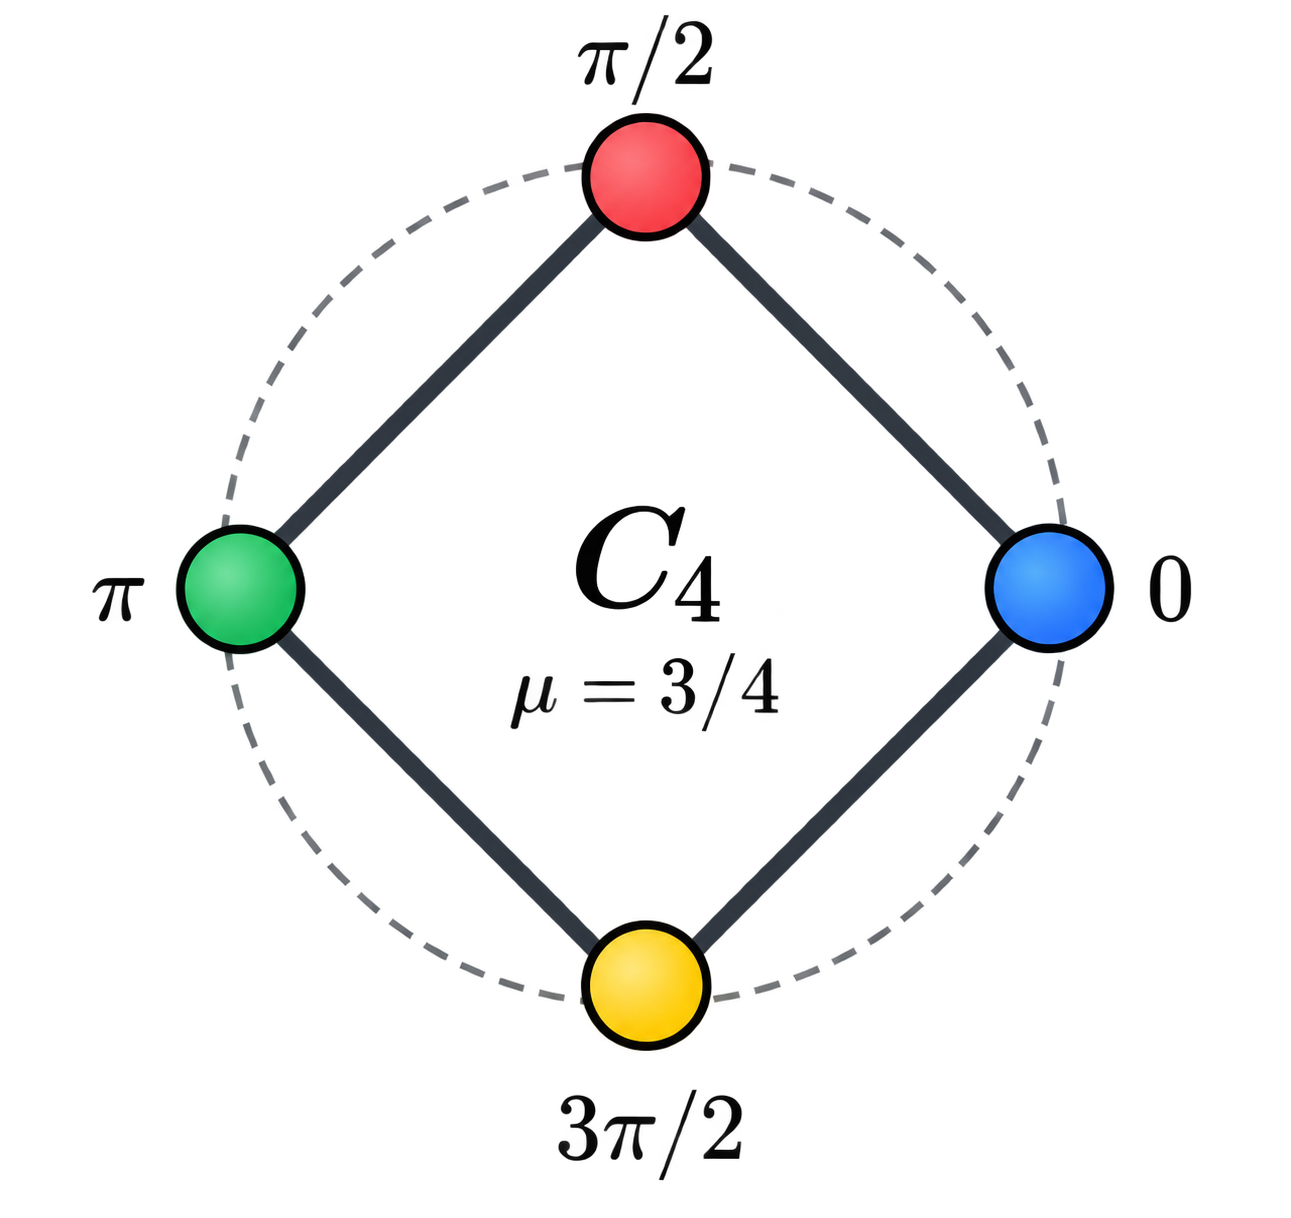
\includegraphics[width=\linewidth/4]{assets/C4.png}
    \caption{Estado \(C_4\).}
    \label{fig:c4}
\end{figure}

Se tiene que $\mu(C_4)=3/4$, pero este estado
no es estable. Kassabov, Strogatz y Townsend
\citep{Kassabov_2021} estudiaron este
estado degenerado, cuya estabilidad no puede
determinarse únicamente mediante el análisis lineal.
Además, $q(C_4)=1$.

Consideremos una conexion interclúster separados en fase en \(\pi/2\). Si perturbamos su fase por \(\epsilon\):

\[
sin(\frac{\pi}{2} + \epsilon) = cos(\epsilon) = 1 - \frac{\epsilon^2}{2} + O(\epsilon^4). 
\]

Por lo que a primer orden, el empuje recibido luego de una perturbación es proporcional a \(cos(\Delta\varphi)\), pero como \(\Delta\varphi = \pi/2\), sera 0.


El hessiano a nivel de clústeres tiene forma

\begin{equation}
    \mathcal{L}(y) = \sum_{a<b}{x_ax_bP_{ab}cos(\varphi_b-\varphi_a)(y_a-y_b)^2}
\end{equation}

En \(C_4\), cada conexión intergrupo tiene coseno 0 y, como grupos opuestos no están conectados directamente, obtenemos \(\mathcal{L}_{C_4}(y)=0\).

\subsection{Perturbaciones de \(C_4\)}

Consideremos
\begin{equation}
    \varphi_a(h) = \frac{\pi}{2}j(a) + hs_a
\end{equation}

Donde \(j(a)\in\{0,1,2,3\}\) identifica el grupo padre, \(s_a\) representa la desviación relativa del clúster \(a\) y \(h>0\) controla la magnitud de la perturbación. En este análisis mantenemos fijas las masas y excluimos
conexiones entre grupos padres opuestos:
\(P_{ab}(h)=0\) si \(j(b)-j(a)\equiv2\pmod4\).
Orientamos los enlaces vecinos de \(V_j\) hacia \(V_{j+1}\),
con índices módulo cuatro.

Por ejemplo, \(S_7\), el testigo de la mejor cota inferior obtenida por \cite{okeeffe20261116densekuramotonetworks}, se puede describir usando nuestra notación con 7 clústers \((-h,h,\pi/2-wh,\pi/2+wh, \pi-h, \pi+h, 3\pi/2)\).

En general, si \(\Delta_{ab} = s_b - s_a\), tenemos una diferencia de fases de \(\pi/2 + h\Delta_{ab}\) obteniendo un \textit{stiffness} de:

\[
\cos(\pi/2+h\Delta_{ab})
=-h\Delta_{ab}+O(h^3).
\]

\subsection{Condiciones de equilibrio}

Buscamos densidades de conexión que hagan estable
la perturbación. Para ello, expandimos
\begin{equation}
    P(h)=P^{(0)}+hP^{(1)}+O(h^2).
\end{equation}

La condición de equilibrio para cada clúster es
\begin{equation}
    F_a(h)=\sum_b x_bP_{ab}(h)
    \sin(\varphi_b(h)-\varphi_a(h))=0,
\end{equation}

Al expandir en potencias de $h$, exigimos
$F_a^{(0)}=F_a^{(1)}=0$.

Sea $V_j$ el conjunto de subclústeres del grupo
padre $j$, con índices módulo cuatro.
A orden cero obtenemos
\begin{equation}
    \sum_{b\in V_{j+1}}x_bP_{ab}^{(0)}
    =
    \sum_{b\in V_{j-1}}x_bP_{ab}^{(0)},
    \qquad a\in V_j.
    \label{eq:equilibrio_cero}
\end{equation}

A primer orden, las fuerzas internas deben ser
compensadas mediante cambios en las densidades:
\begin{equation}
\begin{aligned}
0=F_a^{(1)}
={}&\sum_{b\in V_j}
x_bP_{ab}^{(0)}(s_b-s_a)\\
&+\sum_{b\in V_{j+1}}x_bP_{ab}^{(1)}\\
&-\sum_{b\in V_{j-1}}x_bP_{ab}^{(1)}.
\end{aligned}
\label{eq:equilibrio_uno}
\end{equation}

Ambas condiciones son lineales en las densidades: la primera equilibra las interacciones entre grupos vecinos y la segunda compensa las fuerzas introducidas por la perturbación.

\subsection{Estabilidad a primer orden}

Consideremos perturbaciones colectivas $\eta_j$,
en las que todos los subclústeres del grupo
padre $j$ se desplazan conjuntamente.

Definimos
\begin{equation}
    K_j=
    \sum_{\substack{a\in V_j\\b\in V_{j+1}}}
    x_ax_bP_{ab}^{(0)}(s_b-s_a).
\end{equation}

La expansión del hessiano sobre estos movimientos es
\begin{equation}
    \mathcal{L}_h(\eta)
    =
    -h\sum_{j=0}^{3}
    K_j(\eta_j-\eta_{j+1})^2+O(h^2).
\end{equation}

Las condiciones de equilibrio a orden cero
implican que
\begin{equation}
    \sum_{j=0}^{3}K_j=0.
\end{equation}

Para que exista estabilidad, la matriz del término
de primer orden debe ser semidefinida positiva.
Pero esta matriz tiene traza
$-2\sum_j K_j=0$.

Una matriz semidefinida positiva de traza cero
debe ser nula. Por lo tanto,
\begin{equation}
    K_j=0 \qquad j=0,1,2,3.
    \label{eq:cancelacion_K}
\end{equation}

Es decir, la rigidez colectiva de primer orden
necesariamente se cancela. La estabilidad de los
modos colectivos debe aparecer a segundo orden.

\subsection{Estabilidad a segundo orden}

Para estudiar los modos débiles, consideramos
perturbaciones de la forma
\begin{equation}
    y_a=\eta_{j(a)}+hz_a,
\end{equation}
Para eliminar las redundancias entre movimientos
colectivos y relativos, imponemos
\[
    \sum_{a\in V_j}z_a=0
    \quad\forall j,
    \qquad
    \sum_j\eta_j=0.
\]
donde $\eta_j$ describe el movimiento colectivo
y $z_a$ el movimiento relativo de cada subclúster.

Definimos la energía interna
\begin{equation}
    I=
    \sum_j\sum_{\substack{a<b\\a,b\in V_j}}
    x_ax_bP_{ab}^{(0)}(s_a-s_b)^2.
\end{equation}
y los coeficientes
\begin{equation}
    k_j=
    -\sum_{\substack{a\in V_j\\b\in V_{j+1}}}
    x_ax_bP_{ab}^{(1)}(s_b-s_a).
\end{equation}

Las ecuaciones de equilibrio a primer orden
implican la identidad
\begin{equation}
    \sum_{j=0}^{3}k_j=I.
\end{equation}

La contribución de segundo orden al hessiano
se puede escribir como
\begin{equation}
    \mathcal{L}_h(\eta+hz)
    =
    h^2
    \begin{pmatrix}\eta\\z\end{pmatrix}^{T}
    \mathcal{H}_{\mathrm{lim}}
    \begin{pmatrix}\eta\\z\end{pmatrix}
    +O(h^3),
\end{equation}
donde
\begin{equation}
    \mathcal{H}_{\mathrm{lim}}=
    \begin{pmatrix}
        L_{\mathrm{cut}} & -G^T\\
        -G & L_{\mathrm{in}}
    \end{pmatrix}.
\end{equation}

Aquí $L_{\mathrm{cut}}$ describe la rigidez
entre grupos padres, $L_{\mathrm{in}}$ la rigidez
interna y $G$ el acoplamiento entre ambos tipos
de movimientos.

La condición necesaria de estabilidad es
\begin{equation}
    \mathcal{H}_{\mathrm{lim}}\succeq 0
    \label{eq:hessiano_limite}
\end{equation}
sobre los modos que excluyen la rotación global.

Cuando la rigidez interna es positiva en los
modos relativos, podemos minimizar respecto
de $z$ y obtener el complemento de Schur:
\begin{equation}
    Q_{\mathrm{eff}}
    =
    L_{\mathrm{cut}}
    -G^TL_{\mathrm{in}}^\dagger G.
\end{equation}

El término que se resta es semidefinido positivo:
permitir movimientos internos reduce la rigidez
efectiva de los grupos padres.

\subsection{Formulación mediante SDP}

\paragraph{Búsqueda externa.}
Partimos de cuatro grupos de masa $1/4$ asociados a $C_4$.
Exploramos los quince subconjuntos no vacíos de grupos que
pueden dividirse en dos masas iguales con desviaciones
opuestas, y añadimos divisiones desiguales independientes.
En una familia adicional impusimos las simetrías de $C_4$
que preservan cada partición. Optimizamos las masas y
desviaciones mediante SLSQP y refinamientos con
Nelder--Mead, resolviendo el SDP para cada geometría. Posteriormente exploramos particiones de hasta dieciséis
clústeres. El mejor resultado se obtuvo refinando en
aritmética exacta el patrón observado de tres pares y un
clúster único, seguido de una perturbación racional hacia
el interior de la región estable.

\paragraph{Optimizacion interna.}
Para masas, desviaciones y soporte fijos, las restricciones son lineales o semidefinidas y el problema es convexo. La búsqueda externa modifica la geometría y resuelve este SDP para cada candidato. Finalmente, las mejores soluciones se trasladan a \(h>0\). Los candidatos se validan inicialmente de forma
numérica. Para los mejores resultados se construyen
variantes racionales y se realizan las
certificaciones descritas posteriormente.
Durante la búsqueda fijamos un margen $\gamma>0$.
Denotamos por $\widehat{\mathcal H}_{\mathrm{lim}}$
la matriz de la forma límite en las coordenadas
reducidas anteriores.

\begin{equation}
\begin{aligned}
    \text{maximizar}\quad &\mu_0\\
    \text{sujeto a}\quad
        &F^{(0)}=0,\\
        &F^{(1)}=0,\\
        &K_j=0 \quad \forall j,\\
        &\sum_b x_bP_{ab}^{(0)}
            \geq\mu_0 \quad\forall a,\\
        &0\leq P_{ab}^{(0)}\leq1,\\
        &\hat{\mathcal{H}}_{\mathrm{lim}}\succeq \gamma I.
\end{aligned}
\label{eq:sdp_asintotico}
\end{equation}

Además, imponemos simetría de las matrices,
las restricciones del soporte, rigidez interna
positiva y correcciones $P^{(1)}$ admisibles
respecto de los límites de densidad.

\subsection{Resultados obtenidos}
La construcción $S_7$ de
\cite{okeeffe20261116densekuramotonetworks}
alcanza asintóticamente
\[
    \mu_{S_7}\approx 0.6929077063695864.
\]

Nosotros obtuvimos una familia
de templates estrictos que recuperan \(S_7\) desde perturbaciones de \(C_4\), con
\[
    \lim_{h\to0^+}\mu(T_h)=\mu_0,
    \qquad
    \boxed{\mu_0\ge 0.69290770636958636365.}
\]

\begin{figure}[htbp]
    \centering
    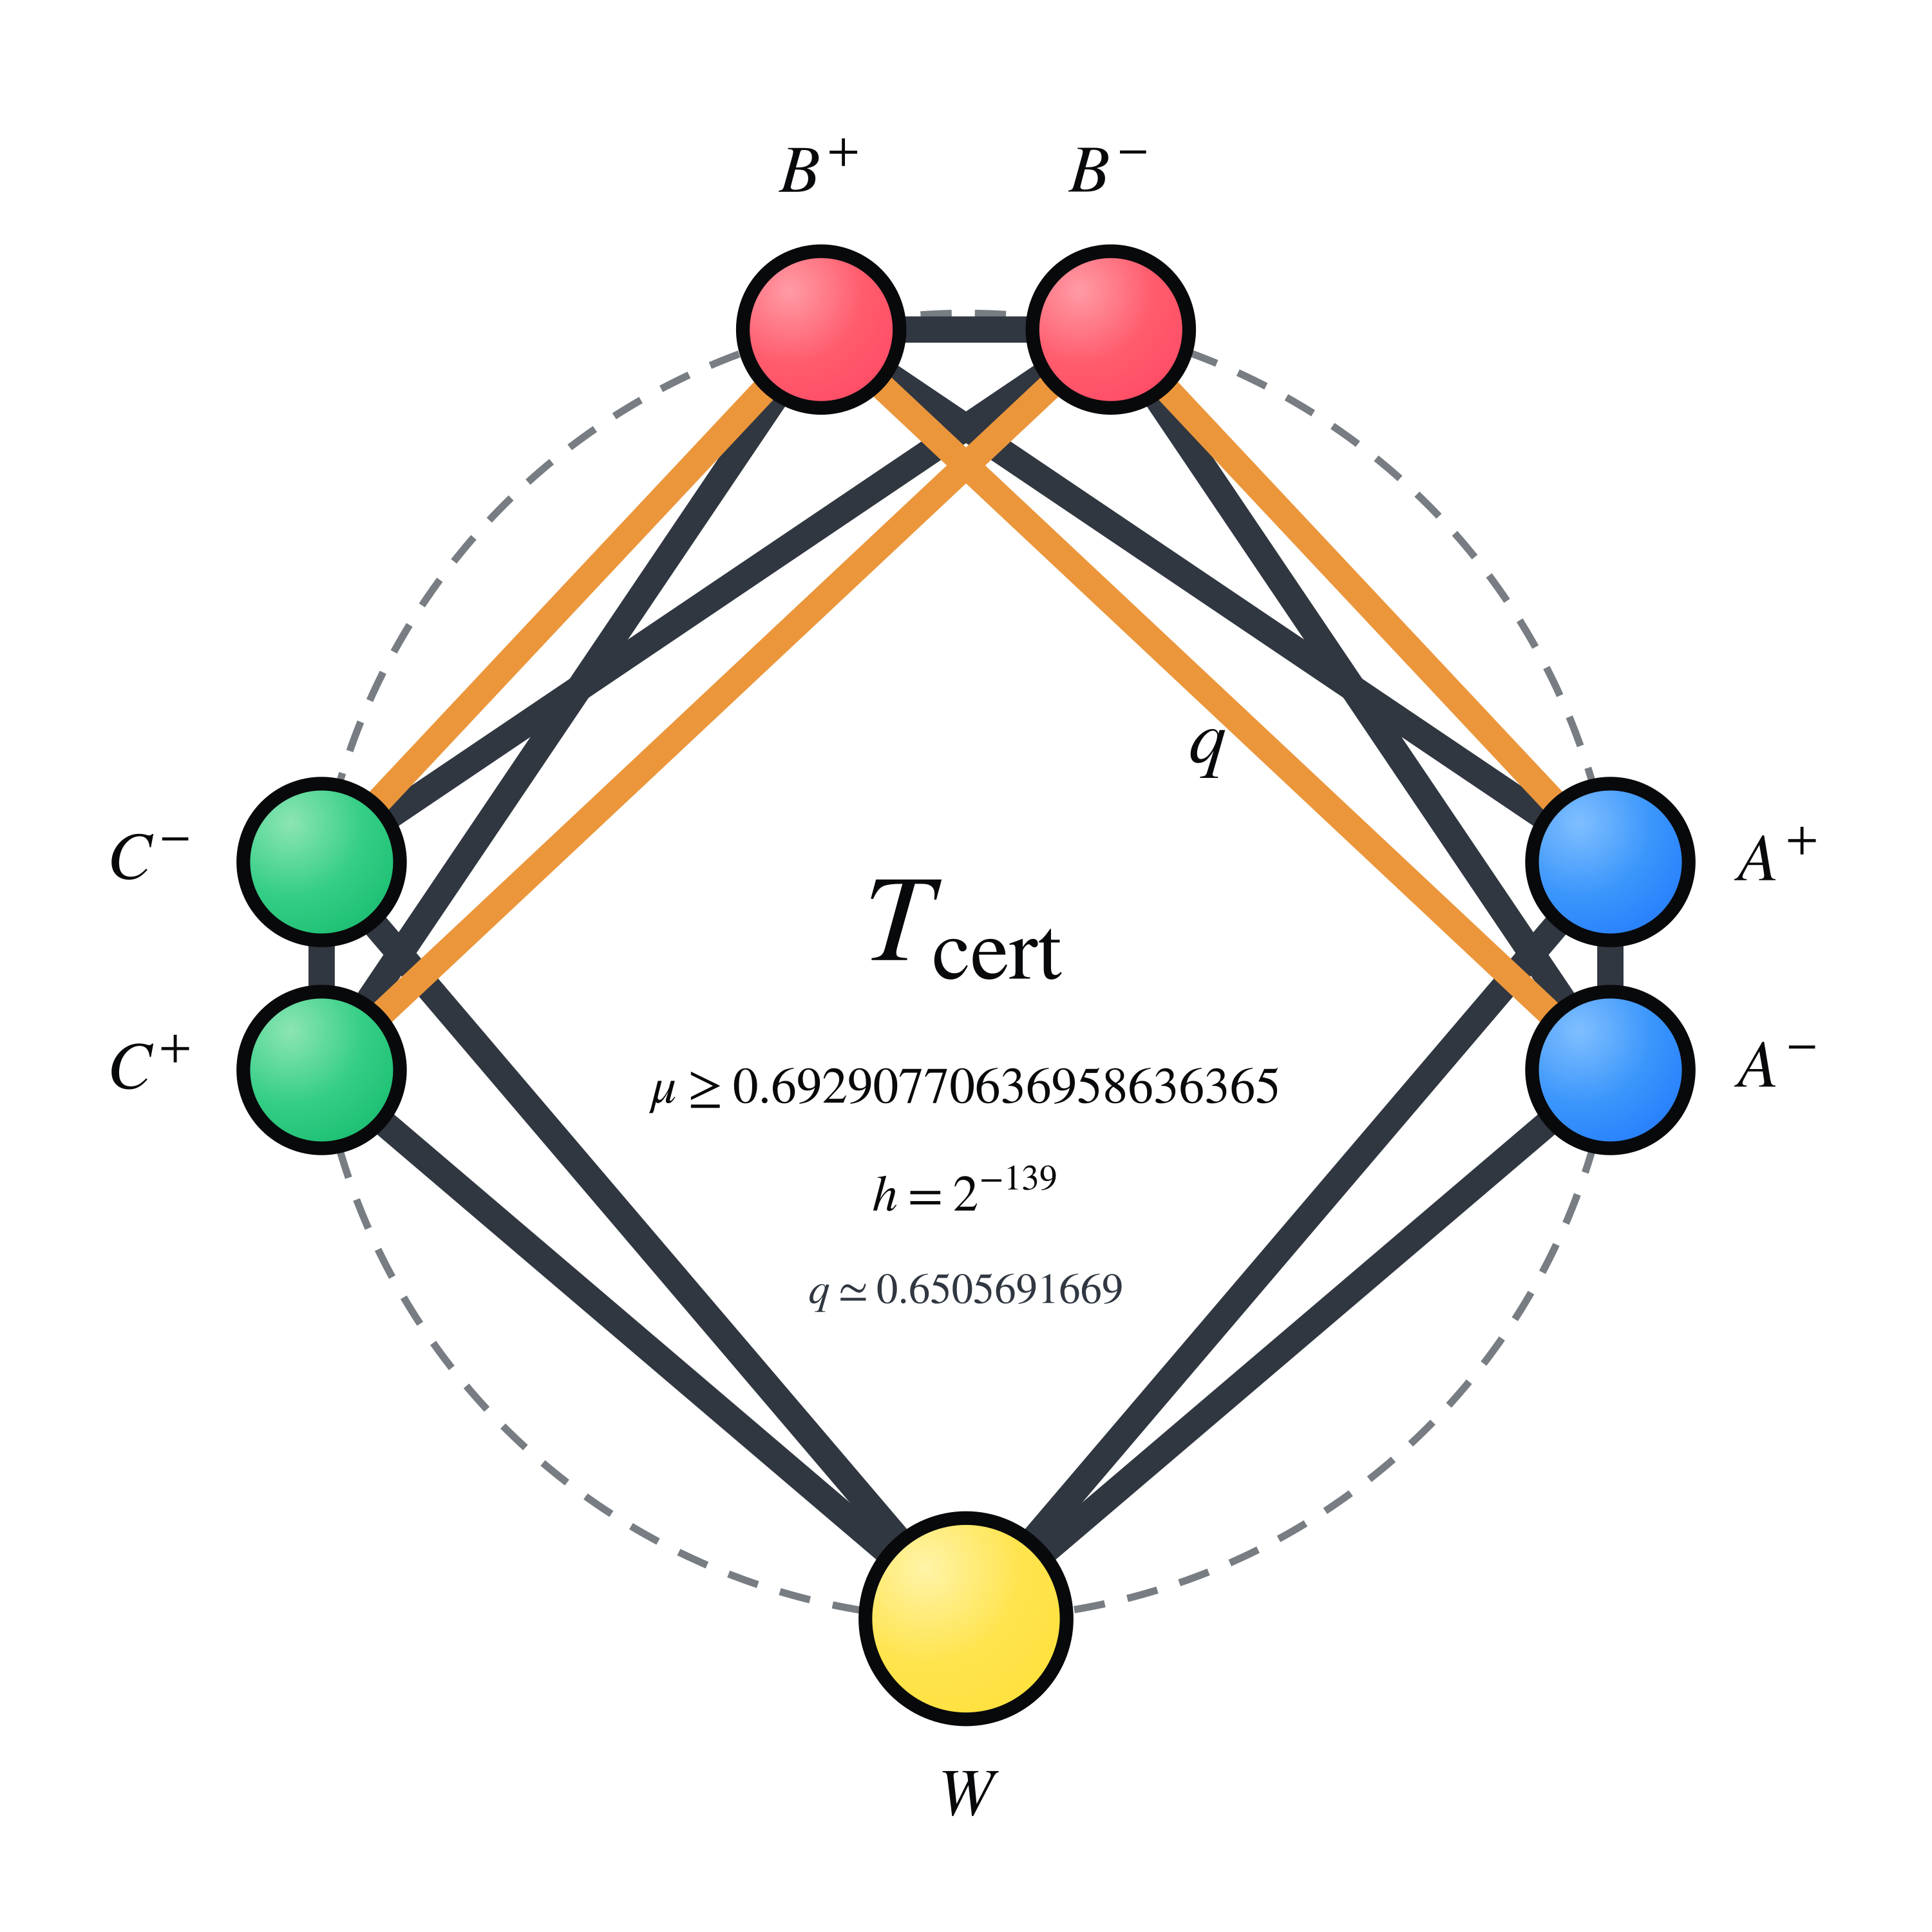
\includegraphics[width=0.3\linewidth]{assets/c4-certified-template-transparent.png}
    \caption{Template certificada, recupera \(S_7\).}
    \label{fig:template_cert}
\end{figure}

Para la familia asintótica se verificaron
exactamente las identidades de equilibrio y,
mediante Cholesky intervalar, la positividad del
hessiano límite; un argumento de levantamiento
establece la existencia para $h>0$ pequeño \citep{okeeffe20261116densekuramotonetworks}.
Para el template finito se verificaron el
equilibrio exacto, la inclusión de Krawczyk
y la estabilidad mediante Cholesky intervalar.

Las certificaciones corresponden a variantes
racionales próximas a las soluciones numéricas.
No superan la cota asintótica publicada ni
demuestran optimalidad global; tampoco se
proporciona una realización explícita en grafos
finitos.

\section{Disponibilidad de datos}\label{da}

El código para reproducir estos experimentos y las demostraciones en Lean se encuentran en \url{https://github.com/LucasGrasso/kuramoto-template-search}.

\section{Reconocimientos}
Los autores agradecen a Y-hat por proporcionar un entorno computacional para el desarrollo de los experimentos computacionales.
La Inteligencia Artificial se usó extensivamente en el desarrollo de los experimentos, de la teoría y sus respectivas demostraciones, utilizándose los modelos Sol 6.1 vía ChatGPT y Argon 4 via Gemini. 


\bibliography{bibliography}


\end{document}